\chapter{Implementation and Testing}

Give a general description of the functionality, context, and design of your project.
Provide any background information if necessary.

\section{Algorithm Design}
Mention the algorithm(s) used in your project to get the work done with regards to major modules. Provide a pseudocode explanation regarding the functioning of the core features. Be sure to use the correct syntax and semantics for algorithm representations. Following are few examples of algorithms/pseudocode. \\

Example:
\begin{figure}[H] % Use 'H' to place the figure exactly here
    \centering
    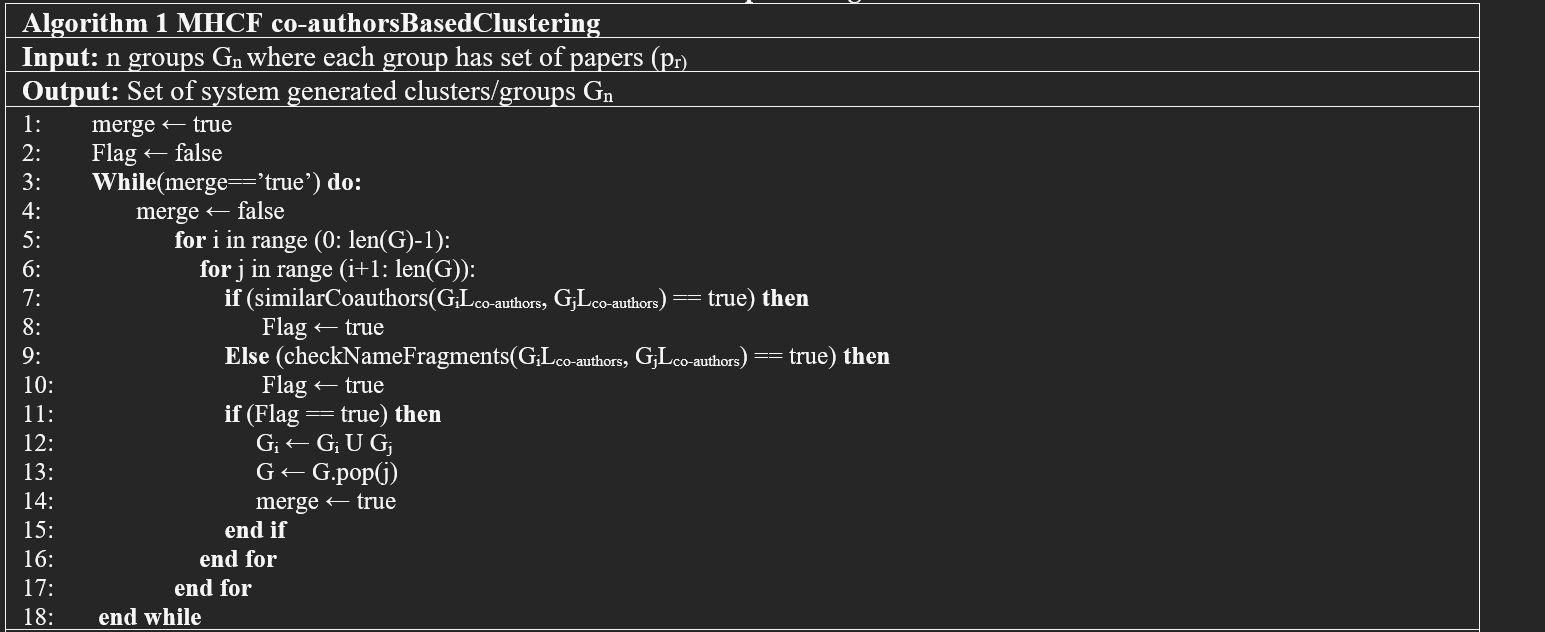
\includegraphics[width=\textwidth]{images/algoexample.png}
    \caption{Example Of Algorithm Design}
    \label{fig:usecase3}
\end{figure}




\section{External APIs/SDKs}
Describe the third-party APIs/SDKs used in the project implementation in the following table. Few examples of APIs are provided in the table.

% Please add the following required packages to your document preamble:
% \usepackage{graphicx}
\begin{table}[!h]
\resizebox{\textwidth}{!}{%
\begin{tabular}{|l|l|l|l|}
\hline
API   and version & Description  & Purpose of   usage & API endpoint/function/class used \\ \hline
Stripe (version 2020-08-27) & Credit Card payment integration & Sandbox used orders payment & stripe.paymentMethods.create \\ \hline
Cloudinary & Image and Video management & Uploading Product Images & https://api.cloudinary.com/v1 \\ \hline
\end{tabular}%
}
\end{table}



\section{Testing Details}
Once the system has been successfully developed, testing has to be performed to ensure that the system working as intended. This is also to check that the system meets the requirements stated earlier. Besides that, system testing will help in finding the errors that may be hidden from the user. The testing must be completed before it is deployed for use. 

\subsection{Unit Testing}
Unit testing is a critical phase in the software development process that involves testing individual components or modules of the system in isolation to ensure that each part functions correctly. The primary goal of unit testing is to validate that each unit of the software performs as designed and meets its specifications. Each unit test is designed to test a specific function or method independently from other components, helping to identify issues directly related to the functionality being tested. Unit tests are often automated, allowing for quick execution and repeatability, which enables frequent running, especially during integration or regression testing, to catch bugs early in the development lifecycle. A well-structured unit testing suite aims to achieve high test coverage, meaning that a significant portion of the codebase is tested, including positive test cases as well as edge cases and error conditions. Furthermore, unit testing provides immediate feedback to developers regarding the quality and reliability of their code, building confidence that changes made during development do not introduce new defects. Additionally, unit tests serve as a form of documentation for the codebase, illustrating how individual units are expected to behave, which makes it easier for new developers to understand the system. Overall, unit testing is an essential practice that contributes to software quality, reliability, and maintainability, ultimately reducing development costs and enhancing the end-user experience. 

Following is the example of Unit testing:

\begin{figure}[H] % Use 'H' to place the figure exactly here
    \centering
    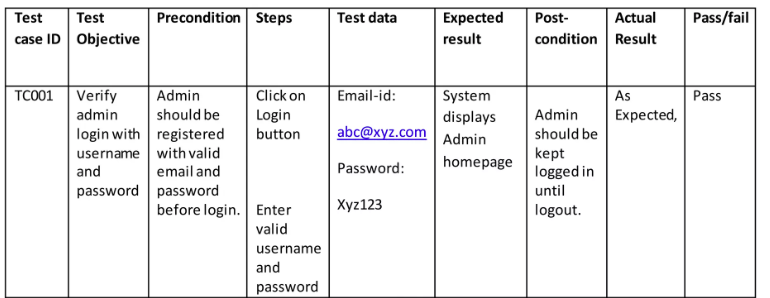
\includegraphics[width=\textwidth]{images/unittesting.png}
    \caption{Example for Unit Testing}
    \label{fig:usecase3}
\end{figure}


